\documentclass[11pt,a4paper]{article}
\usepackage[english]{babel}
\usepackage[utf8]{inputenc}
\usepackage[T1]{fontenc}
\usepackage{graphicx}
\usepackage[hidelinks]{hyperref}
\usepackage{listings}
\usepackage{caption}
\usepackage[left=2cm,text={17cm,24cm},top=3cm]{geometry}


\newcommand{\source}[1]{\caption*{Source: {#1}} }

\bibliographystyle{czechiso}

\begin{document}

\begin{titlepage}
	\begin{center}
	    {\LARGE\textsc{Brno University of Technology}}\\
	    \smallskip
	    {\Large\textsc{Faculty of Information Technology}}\\
	    \bigskip
	    \vspace{\stretch{0.382}}
	    \LARGE{Computer Communications and Networks}\\
	    \smallskip
		\Huge{ARP Scanner}\\
	    \vspace{\stretch{0.618}}
	\end{center}
    {\today \hfill Svätopluk Hanzel}
\end{titlepage}

\tableofcontents

\newpage
\section{Project assignment}
	The main task of this project was to create a network tool capable of scanning local networks using \emph{Address Resolution Protocol} (ARP). Result of such a scan should reveal MAC addresses of computers on network and their corresponding IP addresses.

\section{Address resolution protocol}
	ARP is a critical network protocol for IPv4 networks. It is used for mapping network address to physical address \cite{RFC0826}\cite{Wiki:ARP}.
	\begin{figure}[h]
		\centering
		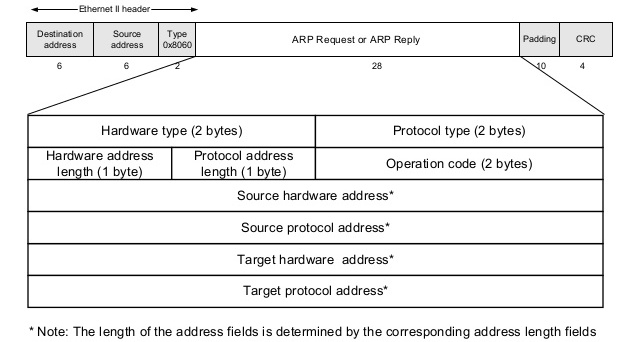
\includegraphics[width=0.7\linewidth]{arp.jpg}
		%\caption{ARP packet format}
		\caption{ARP packet format}
		\label{fig:arp}
		\source{WikiMedia}
	\end{figure}
	
	\subsection{ARP request}
		Whenever computer \emph{A} (IP address 10.0.0.42) wants to communicate with computer \emph{B} (IP address 10.0.0.69), it first has to know the \emph{B}'s physical (\emph{MAC}) address. First, \emph{A} looks into its \emph{ARP cache}, where it has a list of known MAC addresses and corresponding IP addresses \cite{microsoft:arp_cache}. If no record was found for \emph{B}'s IP address, \emph{A} has to issue an \emph{ARP request} before any further requests.
		
		However, since \emph{A} doesn't know \emph{B}'s physical address, this request has to be sent to a \emph{BROADCAST} address, which means that the L2 header's destination field contains \texttt{FF:FF:FF:FF:FF:FF}. Using this approach, all computers in the network receive the ARP request \cite{microsoft:arp_process}.
	\subsection{ARP reply}
		Whenever host receives ARP request, it checks whether his IP address matches the one specified in the ARP request. If it does, its ARP cache is updated with the address mapping of the sender of the ARP request. The host then creates an ARP reply message which contains the requested MAC address and is sent using unicast directly to the sender of the ARP request \cite{microsoft:arp_process}.
		
\newpage
\section{Project solution}
	Solution of this project was rather straight-forward.
	It takes the following steps:
		\begin{enumerate}
			\item Parse arguments
			\item Gather interface information
			\item Send ARP requests and listen for replies
			\item Send ICMPv6 echo request for IPv6 scanning
			\item Generate XML file
		\end{enumerate}
	
	\subsection{Argument parsing}
		The program takes 2 mandatory arguments: \texttt{-i}, which specifies the interface to scan with and \texttt{-f} to specify the XML output file. The argument parsing uses the standard \texttt{getopt} function.
		
	\subsection{Interface information gathering}
		Before any requests can be made, interface informations have to be gathered. This is done in using the \texttt{Interface} class, which discovers all informations about the specified interface including its index, MAC address, all IPv4 addresses and corresponding netmasks and all IPv6 link-local addresses.
		
		All these informations are printed out for debugging/informative reasons.
	
	\subsection{ARP requests processing}
		After all the informations about the specified interface are available, 2 new RAW sockets are opened. One for listening for ARP replies and the other one for sending ARP requests.
		
		A new thread is created for receiving ARP replies. This allows us to receive ARP replies even while other ARP requests are still being sent. In this thread the ARP packets are being received until \texttt{Ctrl+C} is pressed (or \texttt{SIGINT} is sent). Each new host's IP and MAC addresses are then saved for later XML generation.
		
		ARP requests on the other hand are sent in the main thread. ARP requests are sent to all IP addresses in subnet of each address on the interface, i.e. if the interface has 2 IPv4 addresses (\texttt{10.0.0.2/24} and \texttt{10.55.0.3/24}) ARP request is sent to each IP address in the \texttt{10.0.0.0/24} and  the \texttt{10.55.0.0/24} subnet.
		
	\subsection{IPv6 scanning}
		Since IPv6 networks are too big to scan, we cannot simply iterate through all the IPs and send them some request. IPv6 also doesn't have ARP or broadcast. However, in case we need to get all IPv6-enabled hosts in our network we may send a \emph{ICMPv6 echo request} to solicited node address \texttt{ff02::1} to which all devices on our local network belong. After that, all these devices should respond with echo reply \cite{RFC7707}.
		
		In this solution, this technique isn't fully implemented, since Windows machines do not respond to valid multicasted ICMPv6 echo requests and this program sends only valid echo requests.
		
	\subsection{XML generation}
		Once the program received \texttt{SIGINT} signal, it attempts to finish all threads as soon as possible. Once this is done, XML file content is generated and written out to the file.

% References
\newpage
\bibliography{references}

\end{document}

